\documentclass[a4paper,oneside,12pt]{article}
\usepackage{polyglossia}
\usepackage{microtype}
\setdefaultlanguage{english}
%\setotherlanguages{english}
%\usepackage{fontspec}
\usepackage{amsmath}
\usepackage{amssymb}
\usepackage{amsfonts}
\usepackage{mathtools}
\usepackage{xltxtra}
% \usepackage{xunicode}
\defaultfontfeatures{Mapping=tex-text}

\sloppy

\usepackage{ucs}
\usepackage[utf8]{inputenc}
\usepackage[english,hebrew]{babel}
\usepackage{fancyhdr}
\usepackage[colorlinks=true,hidelinks]{hyperref}
\usepackage{ushort}
\usepackage{textcase}
\usepackage{tabularx}
\usepackage{colortbl}
\usepackage{graphicx}
\usepackage[x11names]{xcolor}
\usepackage[left=20mm,right=20mm,top=22mm,bottom=22mm]{geometry}
\setlength{\parindent}{0em}
\definecolor{dark}{RGB}{0,0,0}

\pagestyle{fancy}
\fancyhead{}
\fancyfoot{}
\fancyfoot[RO,RE] {\thepage}
\renewcommand{\headrulewidth}{0pt}
\renewcommand{\footrulewidth}{0pt}

\def\labelitemi  { \raisebox{0.1em} {$\scriptscriptstyle \blacksquare$} }
\def\labelitemii { \raisebox{0.1em} {$\scriptscriptstyle \Box        $} }
%\def\labelitemiii{ \raisebox{0.1em} {$\scriptscriptstyle $} }

\linespread{.7}

\newcommand{\cvpart}[1]{%
\vspace{-1em}%
\section*{\Large\bfseries\MakeTextUppercase{#1}}%
\vspace{-1em}%
\rule{\linewidth}{0.3em}\\[-.3em]%
}

\begin{document}

\begin{centering}
\begin{minipage}{0.70\linewidth}%
\vspace{-3em}{\Huge\bfseries Alexander Zheleznov}

~\\[-.5em]

\hspace{1.9em}\begin{tabularx}{\linewidth}{ll}
{\it E-mail:}		& a.zheleznov@gmail.com\\
{\it Phone:}	        & {\small +972586890662} \\
% ~\\[-1.0em] 
% {\it Address:}	    % & 1118\, Zelenograd\, Apt. 100\\124460\\
%                     & Moscow, Russia\\

~\\[-1.0em]
% {\it Date of birth:}	& 12 June 1985\\
% {\it Marital status:}& married\\
    {\it Citizenship:} & Israeli, Russian \\
    {\it Languages spoken:}& English (upper intermediate), Russian (native), Hebrew (אап)\\
\end{tabularx}
\end{minipage}
% \begin{minipage}{0.23\linewidth}%
% \begin{flushright}
% 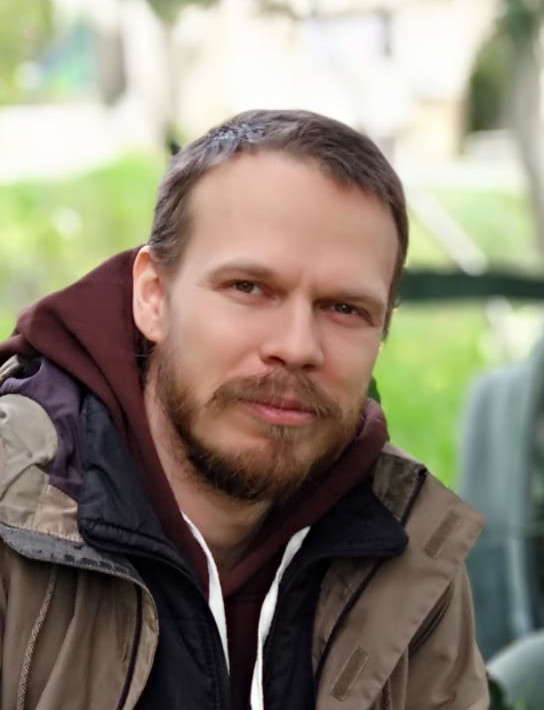
\includegraphics[width=30mm]{me.jpg}
% {%
% \setlength{\fboxsep}{0pt}%
% \setlength{\fboxrule}{0pt}%
% \fbox{
% %    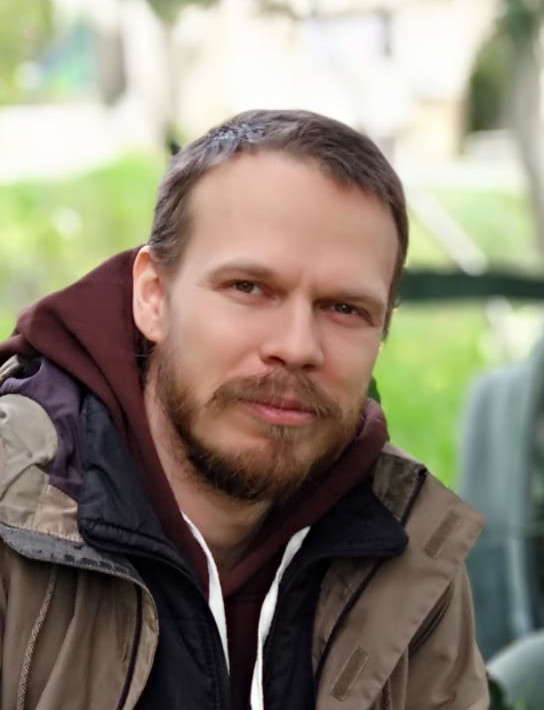
\includegraphics[width=35mm]{me.jpg}
% }
% }%
% \end{flushright}
% \end{minipage}
\end{centering}
~\\[1.5em]


\cvpart{Summary}

I am a C++ and Python Software Developer.
I've recently made my Aliyah and in search of my first job in Israel.

~\\

% \begin{itemize}
% \item Strong knowledge of C/C++ language family and GNU toolchain.
% \item 6 years of experience in UNIX programming environment (GNU/Linux).
% \item Experience in development real-time applications under RTOS (ARINC--429, OS2000).
% \item Experience in development of multithreaded applications (POSIX, Qt).
% \item Experience in development of unit tests(CppUtest, Unity).
    %\item Development of multithreaded applications (libpthread, OpenMP).
%\item Experience in Linux modules development.
%\item Version control systems (git, subversion).
% \item Bash, python and lua scripting, software integration.
%\item Digital signal processing.
%\item Discrete math and algorithm design.
%\item Parallelization and vectorization techniques.
%\item Experience in project management.
% \end{itemize}


\cvpart{Technical skills}
\begin{description}
\item[Programming languages:]~C/C++,~Python,~SQL,~Qt/QML,~Bash,~HTML/CSS/JS.
\item[General developer tools:]~git,~SVN,~vim,~Docker,~Jira,~Latex
% \item[C++ developer tools:]~CMake,~valgrind,~GCC,~clang,~gdb 
\item[General developer skills:]~OOP,~Algorithms,~Unit~Tests,~Debugging,~Agile
\item[Data Science tools: ]~pandas,~NumPy,~scikit-learn,~H{\footnotesize 2}0,~KNIME
\item[General DataScience skills:] ~Machine~Learning,~Data~Visualisation
\item[Advanced user of operating systems:]~Ubuntu,~Arch,~MSDOS,~Windows~98/XP/7/10.
\end{description}

~\\

\cvpart{Education}

\begin{tabularx}{\textwidth}{rX}
  2008~-- 2013:& Saint Petersburg State University (graduate)\\
       % Faculty:& Applied Mathematics and Control Processes\\
    % Department:& Higher Mathematics\\
        Degree:& Specialist's degree in Applied Mathematics and Information Technology\\  
    &~\\[.5em]
          2021:& Financial University under the Government of the Russian Federation  \\
       Subject:& Data Analysis \\ 
         Hours:& 144
\end{tabularx}

~\\

\cvpart{Professional Experience}

% {\bf
% Football Club Sochi, Sochi, Russian Federation. \\ 
% Data Analyst. Internship.\\
% 2022
% }
% \begin{itemize}
%     \item Building ML models for determining outstanding players for the youth league (pandas, KNIME, H2O, scikit-learn, wyscout).
% \end{itemize}
%
{\bf
2021~--- 2022 International Processing Systems.
}
\begin{itemize}
    \item Backend  development for internet banking (C++/Boost).
\end{itemize}

{\bf
2020~--- 2021 Medialooks.
}
\begin{itemize}
    \item Development Windows video tools (MSVisualStudio, ATL/COM).
\end{itemize}

{\bf
2019~--- 2020 Elins.
}
\begin{itemize}
    \item Development of desktop applications for Windows/Linux (Qt, CMake).
    \item Development of UnrealEngine Plugins (UE4, gstreamer, WebRTC).
\end{itemize}

{\bf
2017~--- 2019 Prosoft Biometrics.
}
\begin{itemize}
    \item Development of applications for Raspberry Pi like SoM. (Qt/QML, sqlite, Bash)
    \item Development of web applications. (Python, Flask, AngularJS)
\end{itemize}

{\bf
2012~--- 2016 CSPA Leninetz.
}

\begin{itemize}
    \item Algorithm design and crossplatform implementation for aricraft navigation system.
    % \item Real-time inter process communication(IPC) development for on-board control system (ARINC--429, RapidIO, OS2000, 0S3000).
%\item Cross-platform devdelopment for on board (MIPS64) and testing (x86) systems(C, GNU toolchain).
    \item Developing unit tests for on board code (C, GNU toolchain, CppUtest).
    % \item Porting on-board control system legacy code from MIPS64 to x86 (C, GNU toolchain).
    \item Development of GPS navigation client application (Qt). 
%    \item Debugging and profiling of applications. (gdb, gprof).
%\item API design and writing documentation for interprocessor interaction framework (C99, doxygen).
%\item Software integration~--- developing test stand for on-board system certification (C, shell).
\end{itemize}

\end{document}
